\chapter{Ausarbeitung der Aufgaben}
\section{Impliziter Euler, Octave}
Betrachtet wird ein Transformator, bestehend aus zwei Spulen die über einen Eisenkern miteinander verbunden sind. Der anregende Strom $\textbf{i}(t) = 10[\sin(2\pi ft), 0]^T \SI{}{A}$ hat eine Frequenz von $ f = \SI{50}{\hertz}$. Das semidiskrete magnetoquasistatische Problem

\begin{equation}
	\textbf{M}_\sigma \textbf{\.{a}} + \textbf{\~{C}M}_\nu \textbf{Ca} = \textbf{Xi}(t)
	\label{problem}
\end{equation}

soll im Zeitbereich $T = [0, 0.02]\SI{}{\s}$ gelöst werden. Die Ortsdiskretisierung wird hierbei als schon durchgeführt vorrausgesetzt, deshalb wird im Folgenden nicht darauf eingegangen.

Die Octave-Routine \texttt{trafo\_linear}(siehe Anhang \ref{linear}) erstellt zu Beginn die Materialmatrix $\textbf{M}_\sigma$ und entfernt alle überflüssigen Einträge. Mit dem Aufruf der Funktion \texttt{fit\_operator}(siehe Anhang \ref{fit}) wird die Rotationsmatrix \textbf{C} konstruiert. Mit Hilfe dieser Matrix kann nun die Rotations-Rotations-Matrix $\textbf{K}= \textbf{\~{C}M}_\nu \textbf{C}$ berechnet werden, wobei $\textbf{M}_\nu$ die Reluktivitätsmatrix in Diagonalform darstellt. In diesem Fall wird noch ein linearer Verlauf der Reluktivität angenommen, das heißt die Reluktivität ist an jedem Punkt im Eisenkern zu jeder Zeit gleich.

Die Gleichung (\ref{problem}) wird anschließend mit dem impliziten Eulerverfahren für jeden Zeitschritt im Zeitbereich gelöst. 


\begin{figure}
	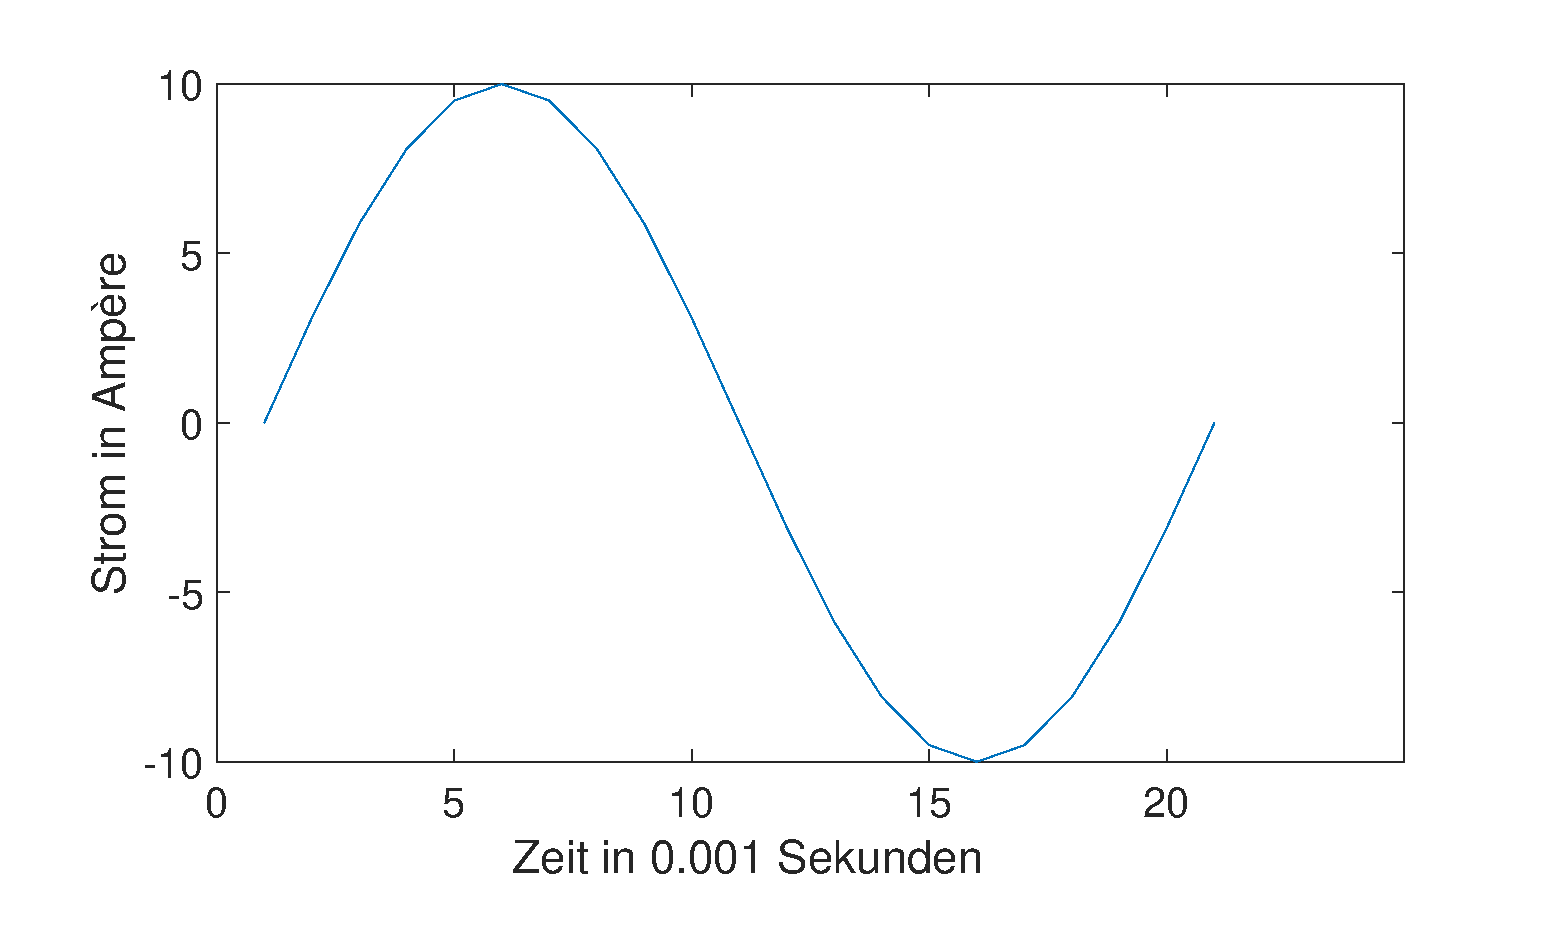
\includegraphics[width=\textwidth]{data/Strom}
	\caption{Anregungsstrom $i(t) = 10\sin(2\pi ft)$}
	\label{fig:Strom}
\end{figure}

Im Postprocessing wird ein Linienplot der Anregung erstellt(siehe Abbildung \ref{fig:Strom}). Außerdem wird für jeden Zeitschritt eine VTK-Datei erstellt zur weiteren Visualisierung des entstehenden Magnetfelds in Paraview.
